\documentclass{article}
\usepackage{pgfplots}
\begin{document}
\thispagestyle{empty}
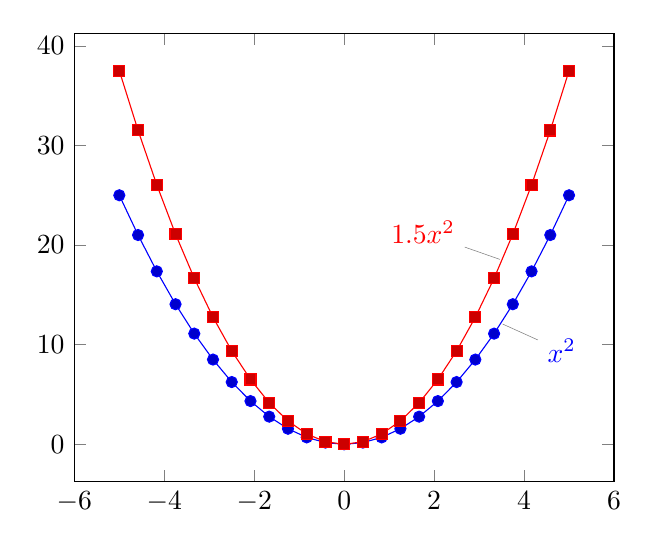
\begin{tikzpicture}
\begin{axis}
\addplot {x^2} node [pos=0.75,pin={-10:$x^2$},inner sep=0pt] {};
\addplot {1.5*x^2} node [pos=0.75,pin={170:$1.5 x^2$},inner sep=0pt] {};
\end{axis}
\end{tikzpicture}


\begin{tikzpicture}
 \begin{axis}[
        axis y line=center,
        axis x line=middle, 
        axis on top=true,
        xmin=-7,
        xmax=7,
        ymin=-4,
        ymax=4,
        clip=false
] 

\addplot[
    mark=none,
    domain=-4:6,
    samples=80,
    red,
    thick,
] {(x<-2)*-2 + (!(x<-2) && (x<3))*x + (!(x<3)) * 3}
    node[pos=0.1,pin=135:{\color{purple}$f(x)=-2$}] {}
    node[pos=0.6,pin=135:{\color{blue}$f(x)=x$}] {}
    node[pos=0.9,pin=135:{\color{green!70!black}$f(x)=3$}] {}
;
\end{axis}
\end{tikzpicture}

\end{document}
